\begin{pastexam}[label={px:ntu-109-bime-ds-03}]{臺大生機所 109 學年度 第 3 題}
（問答）

(20\%) Given the root of a \textbf{binary tree} where each node contains a key, write a pseudocode
program to determine whether it is a \textbf{binary search tree (BST)}. You can use extra space
proportional to the height of the tree.

Note: A node in a \textbf{BST} has two pointers, named `left' and `right', respectively, where the
`left' pointer is used to find the left child of the node and the `right' pointer is used to find
the right child.
\end{pastexam}

\begin{pastsoln}
題目沒有說鍵值會不會重複。 下面照資結書第~9.1~節的定義，鍵值互不相同：每個節點左子樹的鍵都
比它小、右子樹的鍵都比它大。 （若允許重複且規定相等的放右邊，只要把下面的 $\le$、$\ge$ 改成
一邊嚴格一邊不嚴格，見最後一段。）

\textbf{常見的錯}：只檢查每個節點和它的兩個子節點（$x.\mathit{left}.\mathit{key} < x.\mathit{key} <
x.\mathit{right}.\mathit{key}$）是不夠的。 BST 的條件是對\textbf{整棵}子樹說的。 例如下面這棵樹，每個
節點和子節點的關係都對，但 $12$ 在根 $10$ 的左子樹裡卻比 $10$ 大，不是 BST：
\begin{center}
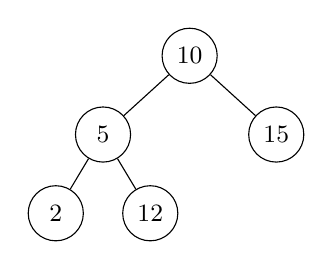
\begin{tikzpicture}[level distance=10mm,
  every node/.style={circle,draw,minimum size=7mm,inner sep=0pt,font=\small},
  level 1/.style={sibling distance=22mm}, level 2/.style={sibling distance=12mm}]
\node {10}
  child {node {5} child {node {2}} child {node {12}}}
  child {node {15}};
\end{tikzpicture}
\end{center}

\textbf{做法：帶著上下界往下走}。 走到節點 $x$ 時，從根到 $x$ 的路上，每往左轉一次就多一個「要比
那個祖先小」的限制，每往右轉一次就多一個「要比那個祖先大」的限制。 這些限制合起來只剩兩個數
有用：最緊的下界 $\mathit{lo}$ 和最緊的上界 $\mathit{hi}$。 所以 $x$ 的子樹是 BST 的條件是：
$\mathit{lo} < x.\mathit{key} < \mathit{hi}$，而且左子樹在範圍 $(\mathit{lo}, x.\mathit{key})$ 內是 BST，
右子樹在範圍 $(x.\mathit{key}, \mathit{hi})$ 內是 BST。

\begin{pseudo}{判斷二元樹是不是 BST}
\Function{Is-BST}{$\mathit{root}$}
    \State \Return \Call{Check}{$\mathit{root}, -\infty, +\infty$}
\EndFunction
\Statex
\Function{Check}{$x, \mathit{lo}, \mathit{hi}$} \Comment{$x$ 的子樹的鍵是否都在 $(\mathit{lo}, \mathit{hi})$ 內且是 BST}
    \If{$x = \NIL$}
        \State \Return \TRUE \Comment{空樹是 BST}
    \EndIf
    \If{$x.\mathit{key} \le \mathit{lo}$ \OR $x.\mathit{key} \ge \mathit{hi}$}
        \State \Return \FALSE
    \EndIf
    \State \Return \Call{Check}{$x.\mathit{left}, \mathit{lo}, x.\mathit{key}$} \AND \Call{Check}{$x.\mathit{right}, x.\mathit{key}, \mathit{hi}$}
\EndFunction
\end{pseudo}
第 8 行的 \AND 是短路求值：左子樹已經不合格就不必再查右子樹。 實作時若沒有 $\pm\infty$，可以傳
「沒有下界／沒有上界」的旗標或空指標。

\textbf{正確性}。 對子樹高度做歸納，證明：\proc{Check}$(x, \mathit{lo}, \mathit{hi})$ 回傳 \TRUE
\textbf{若且唯若} $x$ 的子樹是 BST 而且所有鍵都在 $(\mathit{lo}, \mathit{hi})$ 裡。
\begin{itemize}
\item 空樹：兩邊都成立，回傳 \TRUE。
\item 若回傳 \TRUE：$x.\mathit{key}$ 在範圍內；由歸納假設，左子樹是 BST 且鍵都在
$(\mathit{lo}, x.\mathit{key})$ 裡，也就是都比 $x.\mathit{key}$ 小、而且都在 $(\mathit{lo}, \mathit{hi})$ 裡；
右子樹同理。 這正是「$x$ 的子樹是 BST 且鍵都在範圍內」。
\item 若 $x$ 的子樹是 BST 且鍵都在範圍內：$x.\mathit{key}$ 在範圍內，第 6 行的條件不成立；左子樹
是 BST，鍵都比 $x.\mathit{key}$ 小、也大於 $\mathit{lo}$，由歸納假設左邊的呼叫回傳 \TRUE；右邊同理。
\end{itemize}
以 $(-\infty, +\infty)$ 呼叫，範圍條件自動成立，所以 \proc{Is-BST} 回傳 \TRUE 若且唯若整棵樹是 BST。
上面那棵樹：走到 $12$ 時範圍是 $(5, 10)$，$12 \ge 10$，回傳 \FALSE。

\textbf{複雜度}。 每個節點最多被呼叫一次，每次 $O(1)$，時間 $O(n)$。 遞迴的深度是樹高 $h$，每層
只存 $x$、$\mathit{lo}$、$\mathit{hi}$，額外空間 $O(h)$，符合題目「和高度成正比」的限制。

\textbf{另一種寫法}：BST 的中序走訪是遞增的（資結書定理~9.1），反過來中序走訪遞增的二元樹也一定是
BST（若某節點 $y$ 在 $x$ 的左子樹裡卻 $y.\mathit{key} > x.\mathit{key}$，中序裡 $y$ 排在 $x$ 前面，就不是
遞增）。 所以可以做一次遞迴的中序走訪，用一個變數記上一個走到的鍵 $\mathit{prev}$，每走到一個節點
檢查 $x.\mathit{key} > \mathit{prev}$。 空間同樣是遞迴深度 $O(h)$，不要把整個中序序列存進陣列（那是
$O(n)$ 空間，不符合題目要求）。 允許重複鍵、相等的放右子樹時，改成檢查
$\mathit{lo} \le x.\mathit{key} < \mathit{hi}$ 即可（上下界寫法），中序寫法則改成「不遞減」也不夠，要用上下界。
\end{pastsoln}
